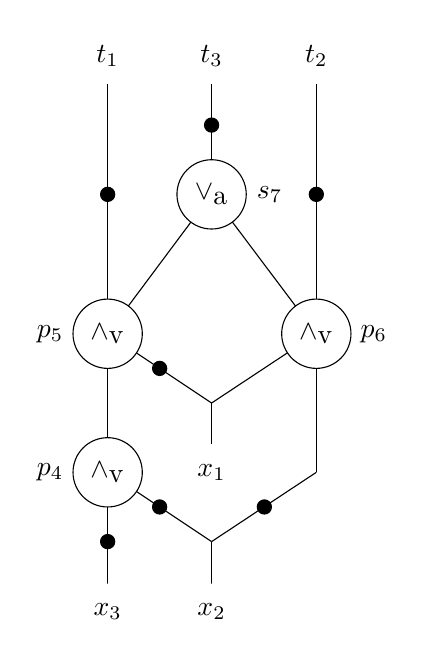
\begin{tikzpicture}
\definecolor{fillcolor}{RGB}{255,255,255}
\definecolor{highcolor}{RGB}{0,0,0}
\definecolor{lowcolor}{RGB}{0,0,0}
\definecolor{neutralcolor}{RGB}{0,0,0}
\definecolor{pathcolor}{RGB}{0,0,0}
\definecolor{background}{RGB}{225,225,225}
\draw (0.44,7.41) [thin,neutralcolor] -- (0.44,3.88);
\draw [fill=neutralcolor,draw=neutralcolor] (0.44,5.65) circle [radius=0.09];
\draw (1.76,7.41) [thin,neutralcolor] -- (1.76,5.65);
\draw [fill=neutralcolor,draw=neutralcolor] (1.76,6.53) circle [radius=0.09];
\draw (3.09,7.41) [thin,neutralcolor] -- (3.09,3.88);
\draw [fill=neutralcolor,draw=neutralcolor] (3.09,5.65) circle [radius=0.09];
\draw (1.76,5.65) [thin,neutralcolor] -- (0.44,3.88);
\draw (1.76,5.65) [thin,neutralcolor] -- (3.09,3.88);
\draw (0.44,3.88) [thin,neutralcolor] -- (1.76,3.00);
\draw [fill=neutralcolor,draw=neutralcolor] (1.10,3.44) circle [radius=0.09];
\draw (0.44,3.88) [thin,neutralcolor] -- (0.44,2.12);
\draw (3.09,3.88) [thin,neutralcolor] -- (1.76,3.00);
\draw (3.09,3.88) [thin,neutralcolor] -- (3.09,2.12);
\draw (1.76,3.00) [thin,neutralcolor] -- (1.76,2.12);
\draw (0.44,2.12) [thin,neutralcolor] -- (0.44,0.35);
\draw [fill=neutralcolor,draw=neutralcolor] (0.44,1.24) circle [radius=0.09];
\draw (0.44,2.12) [thin,neutralcolor] -- (1.76,1.24);
\draw [fill=neutralcolor,draw=neutralcolor] (1.10,1.68) circle [radius=0.09];
\draw (3.09,2.12) [thin,neutralcolor] -- (1.76,1.24);
\draw [fill=neutralcolor,draw=neutralcolor] (2.43,1.68) circle [radius=0.09];
\draw (1.76,1.24) [thin,neutralcolor] -- (1.76,0.35);
\draw [thin,fill=fillcolor,draw=fillcolor] (0.44,7.41) circle [radius=0.35];
\node at (0.44,7.41) {$t_1$};
\draw [thin,fill=fillcolor,draw=fillcolor] (3.09,7.41) circle [radius=0.35];
\node at (3.09,7.41) {$t_2$};
\draw [thin,fill=fillcolor,draw=fillcolor] (1.76,7.41) circle [radius=0.35];
\node at (1.76,7.41) {$t_3$};
\draw [thin,fill=fillcolor,draw=neutralcolor] (1.76,5.65) circle [radius=0.44];
\node at (1.76,5.65) {$\lor_{\textrm{a}}$};
\draw [thin,fill=fillcolor,draw=neutralcolor] (0.44,3.88) circle [radius=0.44];
\node at (0.44,3.88) {$\land_{\textrm{v}}$};
\draw [thin,fill=fillcolor,draw=neutralcolor] (3.09,3.88) circle [radius=0.44];
\node at (3.09,3.88) {$\land_{\textrm{v}}$};
\draw [thin,fill=fillcolor,draw=neutralcolor] (0.44,2.12) circle [radius=0.44];
\node at (0.44,2.12) {$\land_{\textrm{v}}$};
\draw [thin,fill=neutralcolor,draw=neutralcolor] (1.76,3.00) circle [radius=0.00];
\node at (1.76,3.00) {};
\draw [thin,fill=neutralcolor,draw=neutralcolor] (1.76,1.24) circle [radius=0.00];
\node at (1.76,1.24) {};
\draw [thin,fill=neutralcolor,draw=neutralcolor] (3.09,2.12) circle [radius=0.00];
\node at (3.09,2.12) {};
\draw [thin,fill=fillcolor,draw=fillcolor] (1.76,2.12) circle [radius=0.35];
\node at (1.76,2.12) {$x_1$};
\draw [thin,fill=fillcolor,draw=fillcolor] (1.76,0.35) circle [radius=0.35];
\node at (1.76,0.35) {$x_2$};
\draw [thin,fill=fillcolor,draw=fillcolor] (0.44,0.35) circle [radius=0.35];
\node at (0.44,0.35) {$x_3$};
\node [right] at (2.21,5.65) {$s_7$};
\node [right] at (3.53,3.88) {$p_6$};
\node [left] at (0.00,3.88) {$p_5$};
\node [left] at (0.00,2.12) {$p_4$};
\end{tikzpicture}%%
